\paragraph{Optimality condition}

Given a spanning tree $T$, an \textbf{edge} $e \notin T$ is \definitionWithSpecificIndex{cost decreasing}{Edge cost decreasing} if when $e$ is added to $T$ it creates a cycle $C$ with $C \subseteq T \cup \left\{e\right\}$ and $\exists f \in C \setminus \left\{e\right\}$ such that $c_{e} < c_{f}$.
\begin{figure}[!htp]
    \centering
    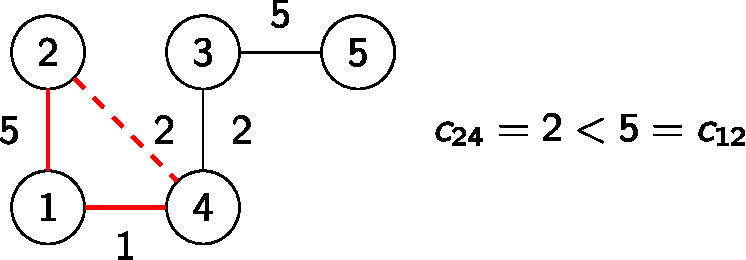
\includegraphics[width=.5\textwidth]{img/trees-opt-condition.pdf}
\end{figure}

\noindent
Because $c\left(T \cup \left\{e\right\} \setminus \left\{f\right\}\right) = c\left(T\right) + c_{e} - c_{f}$, if $e$ is cost decreasing, then:
\begin{equation*}
    c\left(T \cup \left\{e\right\} \setminus \left\{f\right\}\right) < c\left(T\right)
\end{equation*}
\begin{theorem}[Tree optimality condition]
    A tree $T$ is of minimum total cost if and only if no cost-decreasing edge exists.
\end{theorem}
\begin{proof}
    $\Rightarrow$ If a cost-decreasing edge exists, then $T$ is not of minimum total cost.

    $\Leftarrow$ if no cost-decreasing edge exists, then $T$ is of minimum total cost. Let $T^{*}$ be a minimum cost spanning tree found by Prim's algorithm. It can be verified that, by exchanging one edge at a time, $T^{*}$ can be iteratively transformed into $T$ without modifying the total cost. Thus, $T$ is also optimal.
\end{proof}

\noindent
Testing optimality is quite simple. The optimality condition allows to verify whether a spanning tree $T$ is optimal: it suffices to check that each $e \in E \setminus T$ is not a cost-decreasing edge.